\section{Ряды Фурье}

\begin{Def}
	Если у функции $f(x)$ на $[a;b]$ не бесконечное число разрывов первого рода, а других не имеет, то она называется кусочно-непрерывной (далее к-н)на этом промежутке.\\
	Если функция $f(x)$ к-н на $[a;b]$, то она интегрируема на этом отрезке, т.е. $\exists \quad \int\limits_{a}^{b}f(x)dx, f(x) \in R_[a;b]$
\end{Def}

\begin{Note}~\\
	$\forall f(x),g(x)$ - к-н на $[a;b]$ функций справедливо $F(x) = f(x) \cdot g(x)$ - тоже к-н на $[a;b]$
\end{Note}

\begin{Def}
	Пусть $f(x), g(x)$ - к-н функции на $[a;b]$. Тогда их калярным произведением называется $(f(x);g(x)) = \int\limits_{a}^{b}f(x)g(x)dx$
\end{Def}

\begin{Def}
	Пусть $f(x)$ - к-н функция на $[a;b]$. Тогда нормой функции $\|f(x)\|$ называется $\|f(x)\| = \sqrt{(f(x);f(x))} = \sqrt{\int\limits_{a}^{b}f^2(x)dx}$
\end{Def}

\begin{Def}
	Пусть $f(x), g(x)$ - к-н функции на $[a;b]$, тогда $f(x), g(x)$ называются ортогональными $\Leftrightarrow (f(x),g(x)) = 0$ 
\end{Def}

\begin{Note}(Свойства скалярного произведения функций)\\
	Пусть $f(x), g(x), \phi(x)$ - к-н на $[a;b]$ функции, тогда на $[a;b]$ выполняются следующие свойства:
	\begin{enumerate}
		\item $(f(x);g(x)) = (g(x);f(x))$
		\item $(\lambda f(x);g(x)) = \lambda (f(x);g(x)), \quad \lambda$ - костанта
		\item $(f(x) + \phi (x); g(x)) = (f(x);g(x)) + (\phi (x); g(x))$
		\item $\|f(x)\| \geq 0$
		\item $\|\lambda f(x)\| = \lambda\|f(x)\|, \quad \lambda$ - константа
		\item $\|f(x)+g(x)\| \leq \|f(x)\| + \|g(x)\|$
		\item $\|(f(x);g(x))\| \leq \|f(x)\| \cdot \|g(x)\|$ (Неравенство Буняковского-Коши)
	\end{enumerate}
\end{Note}

\begin{Def}
	Система функций $\{\phi_0, \dots \phi_n \dots\}$ называется ортогональной $\Leftrightarrow \forall i,j \in \bb{N} \cup {0} (i \neq j) \quad (\phi_i;\phi_j) = 0$
\end{Def}

\begin{Th}
	Пусть $f(x)$ - функция, а $\{\phi_0, \dots \phi_n \dots\}$ - система функций, заданные на $[a;b]$. $f(x)$ можно представить в виде ряда $\sum\limits_{k=1}^{n}c_k\phi_k(x)$. Тогда $c_k = \frac{(f;\phi_k)}{\|\phi_k\|^2}$
\end{Th}

\begin{Proof}
	$(f;\phi_k) = (c_0\phi_0 + c_1\phi_1 + \dots + c_k\phi_k + \dots; \phi_k) = c_0(\phi_0;\phi_k) + c_1(\phi_1;\phi_k) + \dots + c_k(\phi_k;\phi_k) + \dots = [\text{в силу ортогональности системы}] = c_0\cdot 0 + c_1 \cdot 0 + \dots + c_k \cdot \|\phi_k\|^2 = c_k \cdot \|\phi_k\|^2 \Rightarrow (f;\phi_k) = c_k \cdot \|\phi_k\|^2 \Rightarrow c_k = \frac{(f;\phi_k)}{\|\phi_k\|^2}$
\end{Proof}

\begin{Def}
	Ряд в условиях теоремы 1 называется обобщённым рядом Фурье по ортогональной системе функций $\{\phi_0, \dots \phi_n \dots\}$
\end{Def}

\begin{Note}
	Тригонометрическая система функций (\{$1, \cos x, \sin x,\\ \cos 2x, \sin 2x, \dots, \cos nx, \sin nx, \dots$\}) ортогональна на $[-\pi;\pi]$
\end{Note}

\begin{Proof}
	Для доказательства этого надо доказать пять равенств:
	\begin{enumerate}
		\item $(1;\cos nx) = 0$
		\item $(1;\sin nx) = 0$
		\item $(\sin nx; \cos kx) = 0$
		\item $(\sin nx; \sin kx) = 0, k \neq n$
		\item $(\cos nx; \cos kx) = 0, k \neq n$
	\end{enumerate}

	\begin{enumerate}
		\item $(1; \cos nx) = \int\limits_{-\pi}^{\pi}\cos nx dx =$ [как интеграл от чётной функции по симметричному промежутку] $= 2\int\limits_{0}^{\pi}\cos nx dx = \frac{2}{n} \sin nx\big|_{0}^{\pi} = 0$
		\item $(1; \sin nx) = \int\limits_{-\pi}^{\pi}\sin nx dx =$ [как интеграл от нечётной функции по симметричному промежутку] $= 0$
		\item $(1; \sin nx) = \int\limits_{-\pi}^{\pi}\sin nx \cdot \cos nx dx =$ [$\sin nx$ - нечётная, $\cos nx$ - чётная $\Rightarrow$ произведение - нечётная $\Rightarrow$ как интеграл от нечётной функции по симметричному промежутку] $= 0$
		\item $(\sin nx; \sin kx) = \int\limits_{-\pi}^{\pi}\sin nx \cdot \sin kx dx =$ [произведение нечётных - чётная $\Rightarrow$ как интеграл от чётной функции по симметричному промежутку] = $2\int\limits_{0}^{\pi}\sin nx \cdot \sin kx dx = 2\int\limits_{0}^{\pi}\frac{1}{2}(\cos((n-k)x) - \cos((n+k)x)dx = \frac{\sin((n-k)x)}{n-k}\big|_{0}^{\pi} - \frac{\sin((n+k)x)}{n+k}\big|_{0}^{\pi} = 0 - 0 = 0$
		\item $(\cos nx; \cos kx) = \int\limits_{-\pi}^{\pi}\cos nx \cdot \cos kx dx =$ [произведение чётных - чётная $\Rightarrow$ как интеграл от чётной функции по симметричному промежутку] = $2\int\limits_{0}^{\pi}\cos nx \cdot \cos kx dx = 2\int\limits_{0}^{\pi}\frac{1}{2}(\cos((n-k)x) + \cos((n+k)x)dx = \frac{\sin((n-k)x)}{n-k}\big|_{0}^{\pi} + \frac{\sin((n+k)x)}{n+k}\big|_{0}^{\pi} = 0 + 0 = 0$
	\end{enumerate}
\end{Proof}

\begin{Def}
	Обобщённый ряд Фурье функции $f(x)$ по тригонометрической системе функций называется тригонометрическим рядом Фурье: $f(x) = \frac{a_0}{2} + \baserow{a_n\cos nx + b_n\sin nx}$
\end{Def}

\begin{Note}
	Коэффициенты тригонометрического ряда Фурье вычисляются по формуле:\\
	$a_n = \frac{1}{\pi}\int\limits_{-\pi}^{\pi}f(x)\cos nx dx$\\
	$b_n = \frac{1}{\pi}\int\limits_{-\pi}^{\pi}f(x)\sin nx dx$
\end{Note}

\begin{Def}
	$f(x)$ - кусочно-монотонна на $[a;b] \Leftrightarrow [a;b]$ можно разбить на конечное число частичных итервалов, на каждом из которых в отдельности $f(x)$ монотонна.
\end{Def}

\begin{Note}
	Если $f(x)$ к-н и кусочно-монотонна на $[a;b]$, то говорят, что она удовлетворяет условиям Дирихле
\end{Note}

\begin{Def}(Периодическое продолжение)
	Пусть $f(x)$ определена на $[a;b]$, тогда введём функцию $F(x)$, такую что $\forall x_0 \in \bb{R} \quad F(x_0) = f(a + (||x_0| - [\frac{|x_0|}{|a-b|}]| \cdot |a-b|))$. Тогда $F(x)$ называется периодическим продолжением $f(x)$.\\
	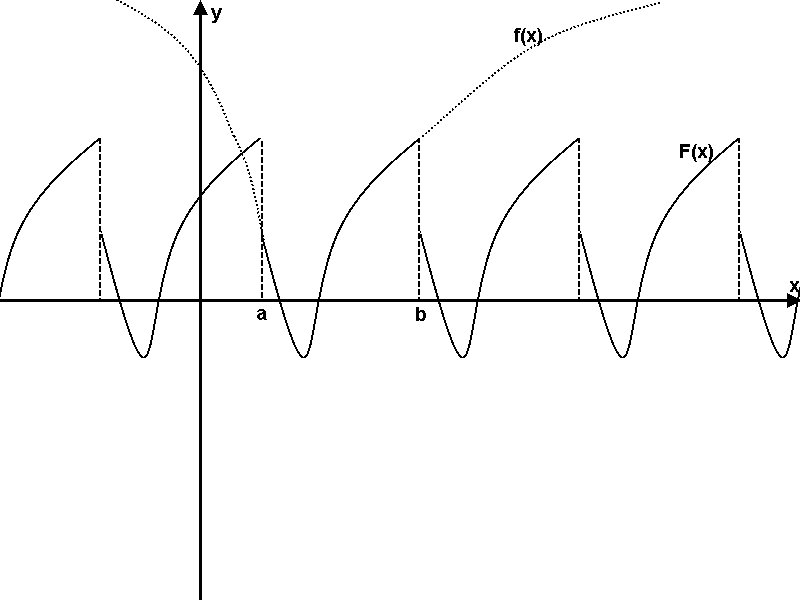
\includegraphics[width=1\textwidth]{pictures/5_2_1.png}
\end{Def}

\begin{Note}
	Периодическое продолжение функции в условиях определения 9 $T$-периодично, $T = |a-b|$
\end{Note}

\begin{Th}
	Пусть $f(x)$ удовлетворяет условиям Дирихле на $[-\pi;\pi]$. Тогда $\forall x_0 \in [-\pi;\pi]$ её ряд Фурье сходится, причём если $x_0$:
	\begin{itemize}
		\item Точка непрерывности $f(x)$, то ряд сходится к $f(x)$
		\item Точка разрыва первого рода к $\frac{f(x-0) + f(x+0)}{2}$
		\item $x_0 = \pm\pi$ к $\frac{f(-\pi+0) + f(\pi-0)}{2}$
	\end{itemize}
	~\\
	Без доказательства
	Также этот ряд сходится к периодическому продолжению $F(x)$ функции $f(x)$на всей числовой оси, а в точках разрыва первого рода к $\frac{F(x-0) + F(x+0)}{2}$
\end{Th}

\begin{Note}
	\begin{itemize}
		\item $f(x)$ - чётная $\Rightarrow b_n = 0 \Rightarrow$ в ряду Фурье только косинусы
		\item $f(x)$ - нечётная $\Rightarrow a_n = 0 \Rightarrow$ в ряду Фурье только синусы
	\end{itemize}
\end{Note}

\begin{Note}
	В случае, если $f(x)$ задана только на промежутке $[0; \pi]$ существует два варианта:
	\begin{enumerate}
		\item Продолжить $f(x)$ на $[-\pi; 0]$ чётным образом $\Rightarrow$ на $[-\pi;\pi]$ функция чётная. В таком случае говорят, что функцию $f(x)$ на $[0;\pi]$ разложили по косинусам
		\item Продолжить $f(x)$ на $[-\pi; 0]$ нечётным образом $\Rightarrow$ на $[-\pi;\pi]$ функция нечётная. В таком случае говорят, что функцию $f(x)$ на $[0;\pi]$ разложили по синусам
	\end{enumerate}
\end{Note}

\begin{Note}
	Пусть $f(x)$ удовлетворяет условиям Дирихле на $[-l;l]$. Тогда разложение $f(x)$ выглядит следующим образом:
	$$
	f(x) = \frac{a_0}{2} + \baserow{a_n\cos(\frac{nx\pi}{l}) + b_n\sin(\frac{nx\pi}{l})}
	$$
	$$
	a_n = \frac{1}{l}\int_{-l}^{l}f(x)\cos(\frac{nx\pi}{l})dx; \quad b_n = \frac{1}{l}\int_{-l}^{l}f(x)\sin(\frac{nx\pi}{l})dx
	$$
\end{Note}

\begin{Proof}
	Введём $t = \frac{x\pi}{l} \Rightarrow t \in [-\pi;\pi]$ и функцию $F(t(x)) = f(x) \forall x \in [-l;l]$. $F(t)$ удовлетворяет условиям Дирихле на $[-\pi;\pi] \Rightarrow\\
	\Rightarrow F(t) = \frac{a_0}{2} + \baserow{a_n\cos(nt) + b_n\sin(nt)}$, где $a_n = \frac{1}{\pi}\int\limits_{-\pi}^{\pi}F(t)\cos(nt) dt$; $b_n = \frac{1}{\pi}\int\limits_{-\pi}^{\pi}F(t)\sin(nt) dt$\\
	$t \rightarrow x \Rightarrow F(t) \rightarrow f(x)$\\
	$f(x) = \frac{a_0}{2} + \baserow{a_n\cos(\frac{nx\pi}{l}) + b_n\sin(\frac{nx\pi}{l})}$;\\
	$a_n = \frac{1}{\pi}\int\limits_{-\pi}^{\pi}F(t)\cos(nt)dt = \frac{1}{\pi}\int\limits_{-l}^{l}f(x)\cos(\frac{nx\pi}{l})\cdot \frac{\pi}{l}dx = \frac{1}{l}\int\limits_{-l}^{l}f(x)\cos(\frac{nx\pi}{l})dx$\\
	$b_n = \frac{1}{\pi}\int\limits_{-\pi}^{\pi}F(t)\sin(nt)dt = \frac{1}{\pi}\int\limits_{-l}^{l}f(x)\sin(\frac{nx\pi}{l})\cdot \frac{\pi}{l}dx = \frac{1}{l}\int\limits_{-l}^{l}f(x)\sin(\frac{nx\pi}{l})dx$
\end{Proof}

\begin{Note}
	Пусть $f(x)$ определена и удовлетворяет условиям Дирихле на $[0;l]$. Тогда:
	\begin{itemize}
		\item её разложение по косинусам на $[0;l]$: $f(x) = \frac{a_0}{2} + \baserow{a_n\cos(\frac{nx\pi}{l})}, a_n = \frac{2}{l} \int\limits_{0}^{l}f(x)\cos(\frac{nx\pi}{l})dx$
		\item её разложение по синусам на $[0;l]$: $f(x) = \frac{a_0}{2} + \baserow{b_n\sin(\frac{nx\pi}{l})}, b_n = \frac{2}{l} \int\limits_{0}^{l}f(x)\sin(\frac{nx\pi}{l})dx$
	\end{itemize}
\end{Note}